% Compile the complete source directory with XeLaTeX, pdfLaTeX or Tectonic.
% Screenshot and vector-plot assets are distributed beside this source.
\documentclass[11pt,letterpaper]{article}
\usepackage[margin=0.72in]{geometry}
\usepackage[T1]{fontenc}
\usepackage[utf8]{inputenc}
\usepackage{lmodern,microtype,graphicx,xcolor,adjustbox}
\usepackage{booktabs,tabularx,array,enumitem,listings,caption,float}
\usepackage{tikz}
\usetikzlibrary{arrows.meta,positioning}
\usepackage{xurl}
\usepackage[hidelinks]{hyperref}
\usepackage{fancyhdr}
\definecolor{ink}{HTML}{203047}
\definecolor{cloudblue}{HTML}{1967D2}
\definecolor{pale}{HTML}{F3F6FA}
\definecolor{green}{HTML}{137333}
\hypersetup{pdftitle={CS528 Homework 4: VM HTTP Service and Pub/Sub Reporter},pdfauthor={Prem Rajendran}}
\pagestyle{fancy}\fancyhf{}
\fancyhead[L]{\small\color{ink} CS528 Homework 4}
\fancyhead[R]{\small\color{ink} Prem Rajendran}
\fancyfoot[C]{\small\thepage}
\setlength{\headheight}{14pt}
\setlength{\parindent}{0pt}
\setlength{\parskip}{5pt}
\setlength{\intextsep}{7pt}
\setlength{\emergencystretch}{2em}
\renewcommand{\arraystretch}{1.16}
\captionsetup{font=small,labelfont=bf,skip=5pt}
\lstset{basicstyle=\ttfamily\footnotesize,backgroundcolor=\color{pale},frame=single,
rulecolor=\color{black!12},breaklines=true,breakatwhitespace=false,columns=fullflexible,
keepspaces=true,showstringspaces=false,aboveskip=6pt,belowskip=6pt,xleftmargin=4pt,xrightmargin=4pt}
\newcolumntype{Y}{>{\raggedright\arraybackslash}X}
\newcommand{\code}[1]{\texttt{\small #1}}
\newcommand{\bucket}{\nolinkurl{cs528-hw3-bu-cs528-prem-project-1791250771}}
\newcommand{\owner}{\nolinkurl{rf6136407ec914afdbeb03a8733430b0b}}
\newcommand{\shot}[3]{\begin{figure}[H]\centering
\includegraphics[width=#2\linewidth]{assets/screenshots/#1}
\caption{#3}\end{figure}}
\newcommand{\plotfigure}[2]{\begin{figure}[H]\centering
\includegraphics[width=\linewidth]{assets/graphs/#1.pdf}\caption{#2}\end{figure}}
\newcommand{\newreportpage}[1]{\clearpage\section{#1}}
\title{\vspace{-1.1cm}\textbf{CS528 Homework 4}\\[4pt]\large HTTP file service and Pub/Sub reporting on VMs}
\author{Prem Rajendran\\Boston University ID: U99248729}
\date{October 13, 2026}
\begin{document}
\begin{center}
{\LARGE\bfseries CS528 Homework 4}\\[4pt]
{\large HTTP file service and Pub/Sub reporting on VMs}\\[9pt]
Prem Rajendran \quad | \quad Boston University ID: U99248729\\[3pt]
October 13, 2026
\end{center}\vspace{-3pt}

\textbf{Course repository:} \url{https://github.com/Pr3mR4jendran/BU-CS528-Cloud-Computing}

\section{Architecture and configuration}
The HW3 file service is recreated as a threaded Python HTTP server on a small Compute
Engine VM. GET uses the URL path and POST uses the request payload to select an existing
HTML object. A separate VM consumes forbidden-country events from Pub/Sub and prints
them to stdout. The instructor's Linux client runs on a third VM.

\begin{figure}[H]\centering
\resizebox{\linewidth}{!}{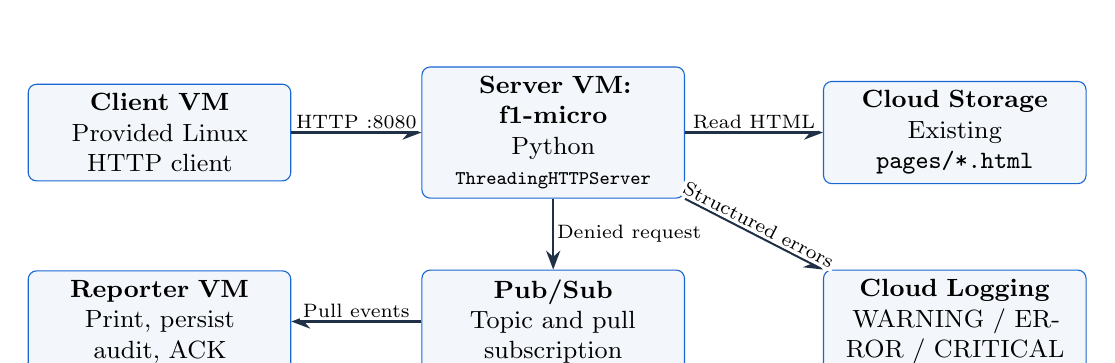
\begin{tikzpicture}[font=\small,
block/.style={draw=cloudblue,fill=pale,rounded corners=3pt,align=center,text width=3.1cm,minimum height=0.95cm},
flow/.style={-{Stealth[length=2.4mm]},thick,draw=ink}]
\node[block] (client) at (0,2.4) {\textbf{Client VM}\\Provided Linux HTTP client};
\node[block] (server) at (5.0,2.4) {\textbf{Server VM: f1-micro}\\Python\\{\scriptsize\ttfamily ThreadingHTTPServer}};
\node[block] (bucket) at (10.1,2.4) {\textbf{Cloud Storage}\\Existing \texttt{pages/*.html}};
\node[block] (reporter) at (0,0) {\textbf{Reporter VM}\\Print, persist audit, ACK};
\node[block] (pubsub) at (5.0,0) {\textbf{Pub/Sub}\\Topic and pull subscription};
\node[block] (logs) at (10.1,0) {\textbf{Cloud Logging}\\WARNING / ERROR / CRITICAL};
\draw[flow] (client) -- node[above,font=\scriptsize,fill=white,inner sep=1pt]{HTTP :8080} (server);
\draw[flow] (server) -- node[above,font=\scriptsize,fill=white,inner sep=1pt]{Read HTML} (bucket);
\draw[flow] (server) -- node[right,font=\scriptsize,fill=white,inner sep=1pt]{Denied request} (pubsub);
\draw[flow] (pubsub) -- node[above,font=\scriptsize,fill=white,inner sep=1pt]{Pull events} (reporter);
\draw[flow] (server.south east) -- node[above,sloped,font=\scriptsize,fill=white,inner sep=1pt]{Structured errors} (logs.north west);
\end{tikzpicture}}
\caption{Three separate VMs. The reporter also writes a deduplicated audit object in the existing bucket under the run's private audit prefix.}
\end{figure}

\begin{tabularx}{\linewidth}{@{}lY@{}}\toprule
Setting & Measured deployment \\ \midrule
Project / location & \code{bu-cs528-prem-project}; \code{us-central1-a}, \code{us-central1} \\
Dataset & \bucket; \code{pages/0.html} through \code{pages/11999.html} \\
Server & \code{cs528-hw4-server}: f1-micro, Debian 12, Python 3.11 \\
Reporter / client & \code{cs528-hw4-reporter}: e2-micro, Debian 12; \code{cs528-hw4-client}: e2-micro, Ubuntu 24.04 \\
Historical endpoint & \nolinkurl{http://104.197.255.22:8080/pages/0.html} \\
Network & Dedicated VPC/subnet; HTTP to server on TCP 8080; IAP SSH on TCP 22 \\
\bottomrule\end{tabularx}

The server address was reserved/static during the experiment. All HW4 infrastructure has
since been deleted; this historical endpoint is no longer a live demonstration. A new
deployment obtains its own address. Ubuntu 24.04 is used for the client because the supplied
binary requires \code{GLIBC\_2.38}; Debian 12 is retained for both services.

\newreportpage{Reproducing the deployment}
\label{sec:reproduce}
Clone the course repository, enter \code{HW-4}, and place the instructor-provided x86-64 Linux
\code{http-client} binary beside \code{deploy.py}. It is excluded from Git. Install Python and
Google Cloud CLI locally. The dataset bucket must already contain the homework HTML files.

\begin{lstlisting}
git clone https://github.com/Pr3mR4jendran/BU-CS528-Cloud-Computing.git
cd BU-CS528-Cloud-Computing/HW-4
gcloud auth login
Copy-Item .\config.example.json .\config.json
python -m venv .venv
& .\.venv\Scripts\python.exe -m pip install -r .\requirements.txt
& .\.venv\Scripts\python.exe -m unittest discover -s tests -v
\end{lstlisting}
Edit \code{config.json} to set the signed-in provisioning account, project, bucket and
dataset prefix. The measured deployment used:
\begin{lstlisting}
{
  "projectId": "bu-cs528-prem-project",
  "account": "premraj@bu.edu",
  "bucketName": "cs528-hw3-bu-cs528-prem-project-1791250771",
  "objectPrefix": "pages/", "maxFileIndex": 11999,
  "region": "us-central1", "zone": "us-central1-a",
  "prefix": "cs528-hw4", "port": 8080,
  "serverMachine": "f1-micro", "reporterMachine": "e2-micro",
  "clientMachine": "e2-micro",
  "clientImageFamily": "ubuntu-2404-lts-amd64",
  "clientImageProject": "ubuntu-os-cloud",
  "httpSourceRanges": ["0.0.0.0/0"]
}
\end{lstlisting}

The provisioning user must be able to enable project APIs, administer Compute resources,
create service accounts, attach them to VMs, change the relevant IAM policies, administer
Pub/Sub, and read the existing dataset. The measured provisioning account had project
Owner. A grader with narrower access also needs the corresponding Compute and service
account permissions and IAP-secured Tunnel User for SSH. The script uses instance metadata
SSH access with OS Login disabled; an organization requiring OS Login needs a deployment
adjustment. These are provisioning privileges, separate from the limited VM runtime roles.

\begin{lstlisting}
& .\.venv\Scripts\python.exe .\deploy.py plan
& .\.venv\Scripts\python.exe .\deploy.py up
if ($LASTEXITCODE -ne 0) { throw 'Deployment incomplete' }
$hw4 = Get-Content .\state.json -Raw | ConvertFrom-Json
$hw4.serverUrl
& .\.venv\Scripts\python.exe .\deploy.py status
\end{lstlisting}
The single \code{up} command creates all three VMs and starts both application services.
It enables the required Compute, IAM, Storage, Pub/Sub, Logging, IAP and Resource Manager
APIs, reserves the server IP, applies scoped IAM, and waits for server/reporter readiness.
Generated startup scripts embed the application source and configuration in VM metadata,
install dependencies, and enable systemd units. First boot needs no GitHub credentials.
An incomplete deployment can be resumed with the same code/config and state file.

\newreportpage{Runtime identities and least privilege}
\label{sec:iam}
The server and reporter use different dedicated service accounts. Their credentials come
from the VM metadata service; application key files are unnecessary. Both applications run
as the unprivileged Linux user \code{hw4app}. The client VM has no attached service account.

\begin{tabularx}{\linewidth}{@{}p{0.95in}p{1.9in}Y@{}}\toprule
Identity & Granted role & Resource / restriction \\ \midrule
Server & Storage Object Viewer & Existing bucket, conditional read of \code{pages/} objects only \\
Server & Pub/Sub Publisher & \code{cs528-hw4-forbidden} topic only \\
Server & Logs Writer & Project, for the application's structured error logs \\
Reporter & Pub/Sub Subscriber & \code{cs528-hw4-reporter} subscription only \\
Reporter & Storage Object User & Existing bucket, conditional access to \code{hw4-logs/<owner>/} only \\
Client & None & No attached account or application IAM grant \\
\bottomrule\end{tabularx}

The account names are \nolinkurl{cs528-hw4-server@bu-cs528-prem-project.iam.gserviceaccount.com}
and \nolinkurl{cs528-hw4-reporter@bu-cs528-prem-project.iam.gserviceaccount.com}.
The cloud-platform OAuth scope permits API calls; the IAM bindings above limit authorization.
The exact bucket IAM conditions are:
\begin{lstlisting}
// Server: roles/storage.objectViewer
resource.name.startsWith('projects/_/buckets/cs528-hw3-bu-cs528-prem-project-1791250771/objects/pages/')

// Reporter: roles/storage.objectUser
resource.name.startsWith('projects/_/buckets/cs528-hw3-bu-cs528-prem-project-1791250771/objects/hw4-logs/rf6136407ec914afdbeb03a8733430b0b/')
\end{lstlisting}
The server cannot write dataset objects. The reporter's audit access does not extend to
the dataset prefix. Storage Object User is scoped to the audit prefix to support a
generation-checked read/modify/write and retry on concurrent updates.

\shot{bucket-storage-condition.png}{1}{Server bucket role condition restricting object reads to the dataset prefix.}
\shot{reporter-storage-condition.png}{1}{Reporter bucket role condition restricting audit access to this run's owned prefix. The conditions are also transcribed above for legibility.}
Exported policies and VM identities/scopes were verified before cleanup. The appendix shows
project Logs Writer and resource-level Pub/Sub roles. Cleanup removed the runtime grants.

\newreportpage{VM placement, static IP and automatic startup}
\shot{VM-list.png}{1}{All three VMs running in us-central1-a. The client and reporter are distinct from the HTTP server.}
\begin{minipage}[t]{0.49\linewidth}\centering
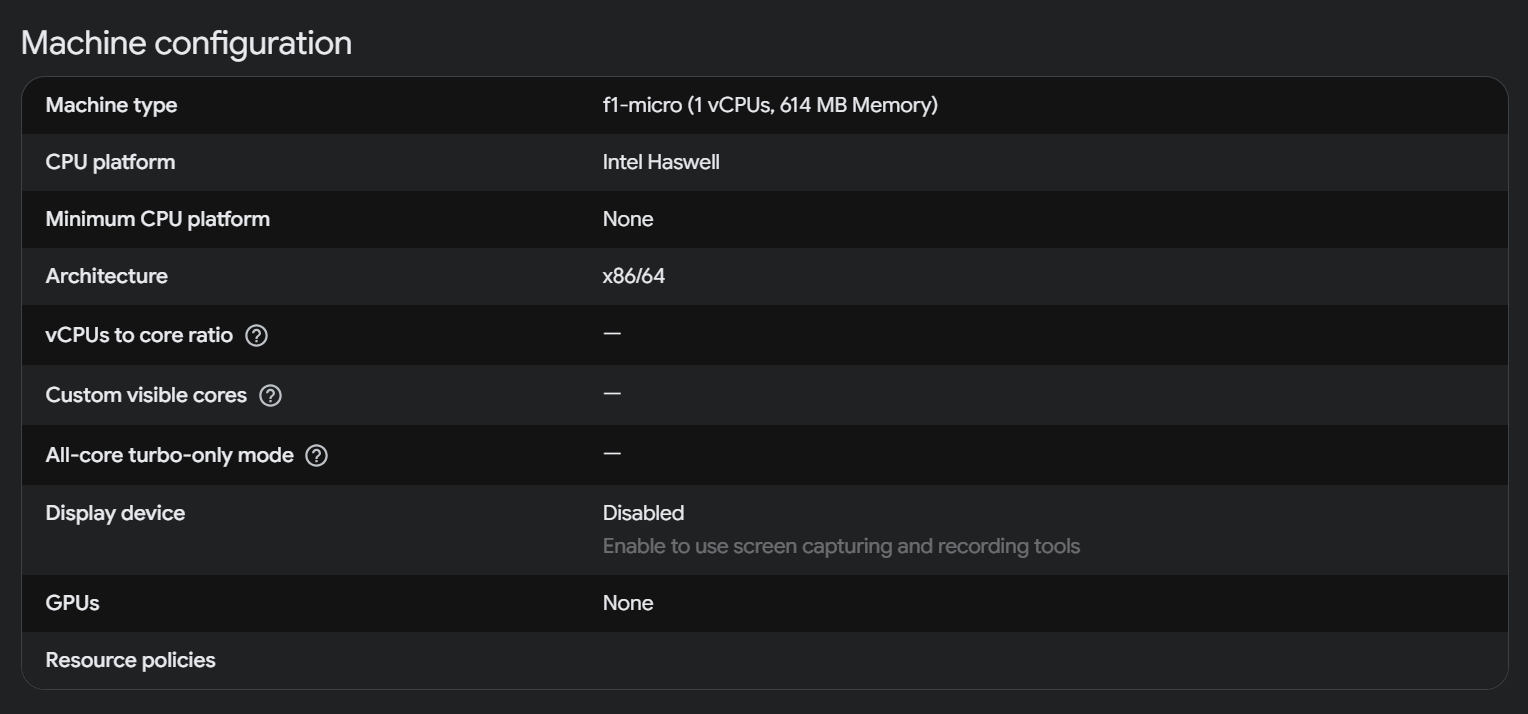
\includegraphics[width=\linewidth]{assets/screenshots/server-config.png}
\captionof{figure}{Server machine configuration: f1-micro.}
\end{minipage}\hfill
\begin{minipage}[t]{0.49\linewidth}\centering
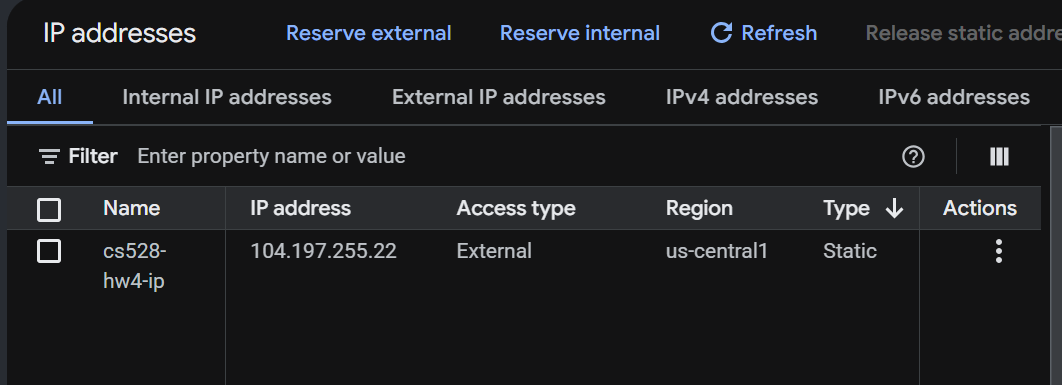
\includegraphics[width=\linewidth]{assets/screenshots/static-IP.png}
\captionof{figure}{Reserved static address attached to the server.}
\end{minipage}

\shot{server-IAM.png}{0.94}{Dedicated server service account attached to the server VM.}
\begin{figure}[H]\centering
\adjincludegraphics[trim={0 0 {.28\width} {.70\height}},clip,width=0.94\linewidth]{assets/screenshots/client-IAM.png}
\caption{Client VM identity panel: no attached service account. The complete screenshot is retained in the source package.}\end{figure}
Startup creates \code{cs528-hw4-server.service} and \code{cs528-hw4-reporter.service}, both
enabled and active. Units depend on network readiness, restart on failure after five
seconds, and use \code{NoNewPrivileges}, \code{PrivateTmp}, \code{ProtectSystem=strict} and
\code{ProtectHome}. Source and runtime configuration live in \code{/opt/cs528-hw4}.

\newreportpage{HTTP behavior and curl verification}
\label{sec:http}
\begin{tabularx}{\linewidth}{@{}>{\raggedright\arraybackslash}p{1.55in}p{0.6in}p{0.8in}Y@{}}\toprule
Request & Status & Severity & Observed behavior \\ \midrule
GET existing file & 200 & -- & Original HTML bytes from Cloud Storage \\
POST filename payload & 200 & -- & Same original HTML bytes \\
GET missing object & 404 & WARNING & Structured \code{file\_not\_found} record \\
PUT, DELETE, HEAD, CONNECT, OPTIONS, TRACE, PATCH & 501 & ERROR & Structured \code{unsupported\_method} record \\
GET with banned X-country & 400 & CRITICAL & Denial log plus Pub/Sub event; no object download \\
\bottomrule\end{tabularx}
Country denial follows the assignment's simulated list: North Korea, Iran, Cuba, Myanmar,
Iraq, Libya, Sudan, Zimbabwe and Syria. It uses the supplied \code{X-country} request header.
The list is an assignment policy, not a claim about current export regulations.

The \code{demos.py} harness ran actual curl requests and saved response headers, bodies,
exit codes and request event IDs. All 19 cases passed: GET, POST, one missing file,
all seven unsupported methods and all nine forbidden countries. All 17 expected
error records were matched to their Cloud Logging severities. GET and POST body hashes
matched the bucket object's SHA-256:
\begin{lstlisting}
c3be7cacaad7e54bac9e5050419002b0545418e31094933b4239813e2a6f2b88
\end{lstlisting}
Run the full demo after deployment; use the new URL from state rather than the historical IP:
\begin{lstlisting}
& .\.venv\Scripts\python.exe .\demos.py
$hw4 = Get-Content .\state.json -Raw | ConvertFrom-Json
$base = $hw4.serverUrl -replace '/pages/0.html$',''
curl.exe -i "$base/pages/12000.html"
curl.exe -i -X PATCH "$base/pages/0.html"
curl.exe -i -H 'X-country: Iran' "$base/pages/0.html"
\end{lstlisting}
POST uses a JSON body such as \code{\{"filename":"pages/0.html"\}} with
\code{Content-Type: application/json}; form and plain-text payloads are also supported.
\shot{request-400-404-500.png}{1}{Saved curl responses: missing file 404, unsupported PATCH 501 and Iran country denial 400.}

\newreportpage{Browser demonstrations}
The browser first loaded the original HTML page from the server. From that same origin,
DevTools \code{fetch} requests exercised GET/POST 200, missing-file 404, PATCH 501 and Iran
400. The console shows the actual returned statuses; its red 404/501/400 messages are the
expected error cases, rather than a failed test harness.
\begin{figure}[H]\centering
\adjincludegraphics[trim={0 {.68\height} {.50\width} 0},clip,width=0.91\linewidth,height=2.3in,keepaspectratio]{assets/screenshots/HTML_render.png}
\caption{Upper-left browser excerpt: HTML rendered at the server's historical static-IP endpoint. The complete screenshot is retained with the source.}\end{figure}
\begin{figure}[H]\centering
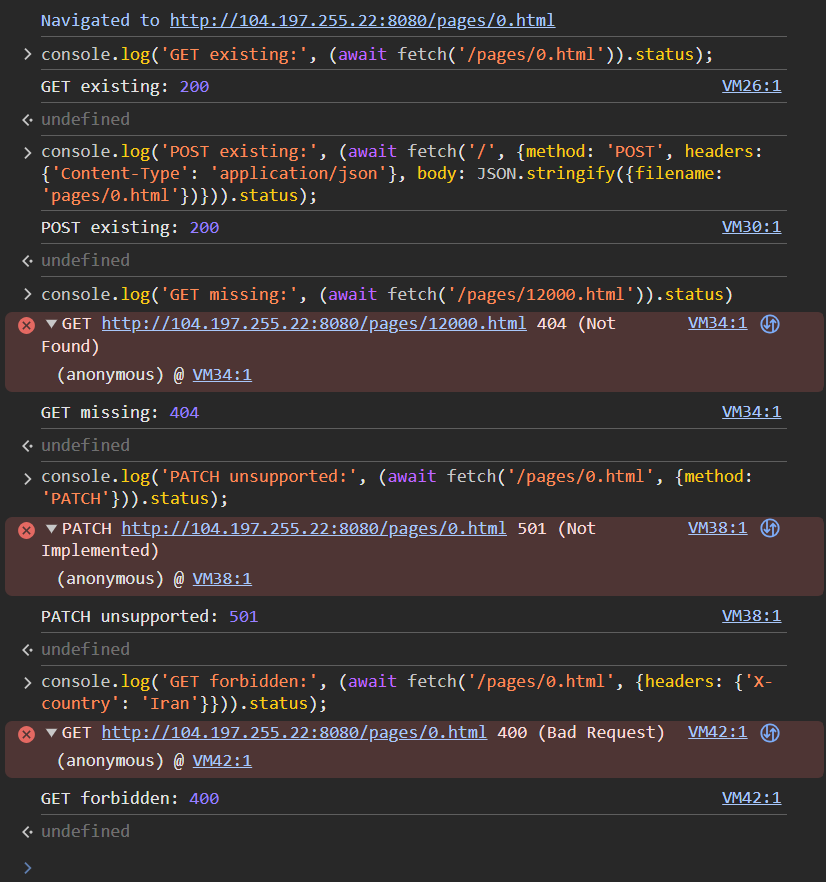
\includegraphics[height=4.85in,keepaspectratio]{assets/screenshots/browser-console-tests.png}
\caption{One browser request for each status case, including both supported methods. GET and POST return 200; the remaining requests return 404, 501 and 400.}\end{figure}

\newreportpage{Structured Cloud Logging: missing and unsupported requests}
The application calls Cloud Logging with a structured JSON payload and an explicit
severity. Records carry \code{event\_id}, method, path, filename, status, country and timestamp.
The two screenshots below show the complete error payload and severity in Logs Explorer.
\begin{figure}[H]\centering
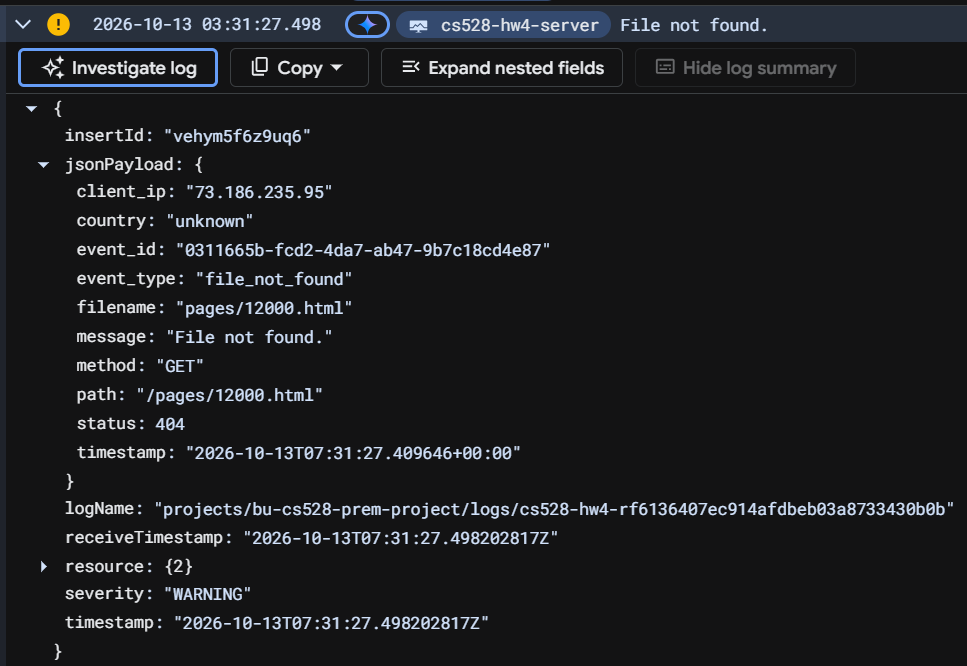
\includegraphics[height=3.25in,keepaspectratio]{assets/screenshots/cloud-request-404.png}
\caption{Missing \code{pages/12000.html}: status 404, event type \code{file\_not\_found}, severity WARNING.}\end{figure}
\begin{figure}[H]\centering
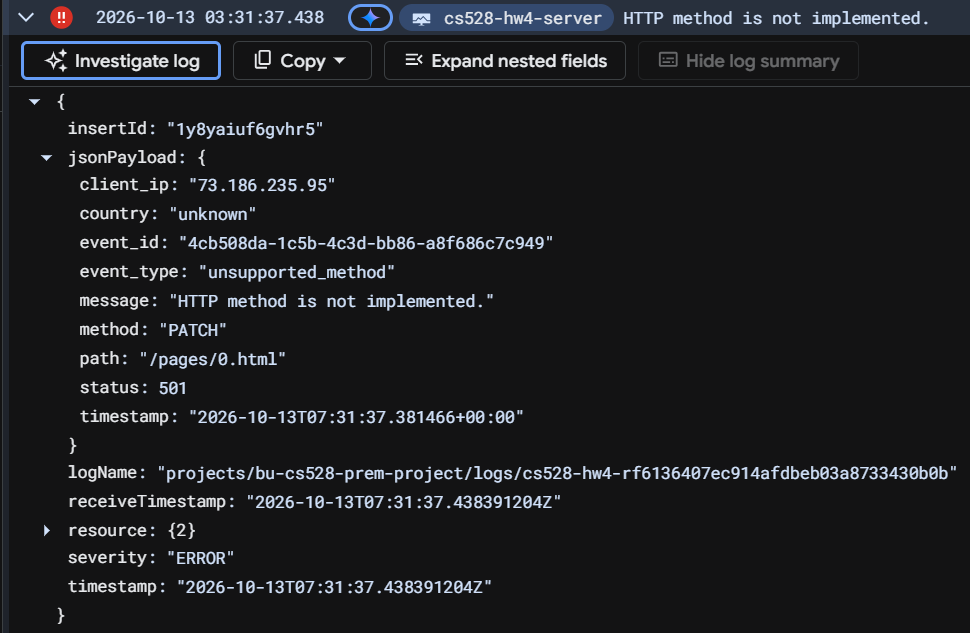
\includegraphics[height=3.15in,keepaspectratio]{assets/screenshots/cloud-request-501.png}
\caption{Unsupported PATCH: status 501, event type \code{unsupported\_method}, severity ERROR.}\end{figure}
The full pre-cleanup export contains 1,833 custom application log entries. The final
collection was not restricted to the first 1,000 entries. These exported records survive
locally even though cleanup deletes this run's custom cloud log.

\newreportpage{Forbidden-country events and reporter delivery}
\begin{figure}[H]\centering
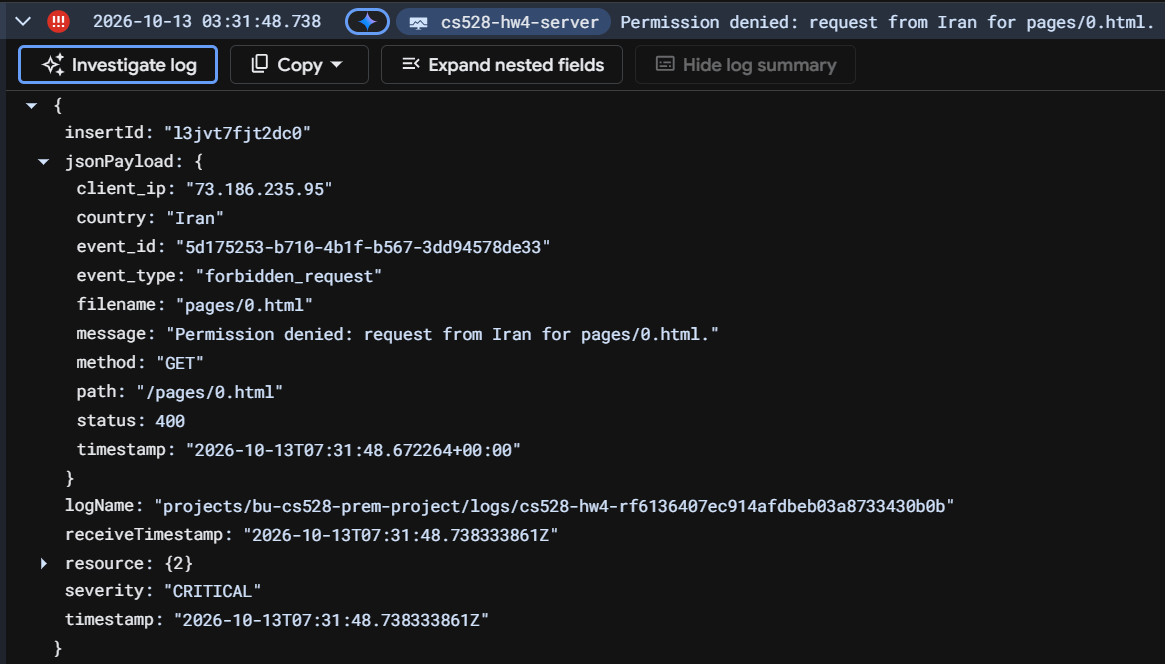
\includegraphics[width=0.83\linewidth]{assets/screenshots/cloud-request-400.png}
\caption{An Iran request is denied with HTTP 400 and a structured CRITICAL Cloud Logging entry.}\end{figure}
For this example, the same event ID appears in the CRITICAL log, the reporter's stdout
and the persisted audit object. The reporter prints an appropriate denial message with
the country and filename. Its stdout record uses WARNING; the server's Cloud Logging
record uses the assignment-required CRITICAL severity.
\begin{lstlisting}
event_id: 5d175253-b710-4b1f-b567-3dd94578de33
country: Iran                    filename: pages/0.html
message: Permission denied: request from Iran for pages/0.html.
pubsub_message_id: 22010629669199521
\end{lstlisting}
\shot{Screenshot 2026-10-13 040250.png}{1}{Saved reporter journal and audit-object lookup for the same event ID. The details are transcribed above for readability.}
The subscriber acknowledges a message only after the audit write and stdout record.
Audit updates use Cloud Storage generation preconditions and deduplicate by event ID,
so a redelivery after an interrupted acknowledgement does not append a second entry.
Before cleanup, all \textbf{1,119} forbidden events from the final stress suite matched
CRITICAL server logs, reporter stdout and exactly one audit entry. The full retained
audit has 1,783 unique events, including earlier demonstrations and trial runs.

\newreportpage{Provided client and service readiness}
\label{sec:client}
\code{run\_client.py} copies/runs the instructor's binary on \code{cs528-hw4-client},
independent of both service VMs. The verified standalone run requested 100 files with
the following remote command:
\begin{lstlisting}
/opt/cs528-hw4/http-client -d 104.197.255.22 -b none -w pages \
  -n 100 -i 11999 -p 8080 -r 0 -t 60 -v

# Local orchestration after up:
& .\.venv\Scripts\python.exe .\run_client.py
\end{lstlisting}
\begin{tabularx}{\linewidth}{@{}lY@{}}\toprule
Check & Latest standalone 100-request result \\ \midrule
Expected / observed responses & 100 / 100 \\
Successful downloads & 94 HTTP 200 responses \\
Expected country denials & 6 HTTP 400 responses; all 6 persisted denials verified \\
Client exit / verification & Exit code 0; \code{passed=true} \\
\bottomrule\end{tabularx}
The 100-request evidence includes compact client output, request IDs, body/type checks,
the command, and a cloud export. Expected country denials are not server-capacity errors.
The result is saved under \nolinkurl{client-100-20261013T074028911477Z}.

\begin{figure}[H]\centering
\adjincludegraphics[trim={0 {.74\height} {.46\width} 0},clip,width=0.94\linewidth]{assets/screenshots/server-logs.png}
\caption{Server startup/status excerpt: the systemd unit is enabled and active. The complete original screenshot is retained in the source package.}\end{figure}
\begin{figure}[H]\centering
\adjincludegraphics[trim={0 {.74\height} {.46\width} 0},clip,width=0.94\linewidth]{assets/screenshots/reporter-logs.png}
\caption{Reporter startup/status excerpt: its own systemd unit is enabled and active. Figure~15 shows received forbidden requests on stdout.}\end{figure}
The deployment command's readiness checks include a real bucket-backed HTTP request,
the reporter's ready message, client bootstrap completion and the supplied binary's help
output. The local test suite also passes all 33 tests, covering real HTTP sockets,
audit behavior, cleanup ownership, sampling and failure accounting. Cloud IAM and
deployment success are supported by live exports, not inferred from mocked local tests.

\newreportpage{Stress-test method and measured results}
\label{sec:stress}
The report uses only the completed \nolinkurl{stress-20261013T155600814186Z} experiment.
One, two, three and four concurrent provided-client processes each ran for \textbf{180 seconds}
on the client VM, separated by 15-second cooldowns. Each process makes sequential requests;
``clients'' describes processes rather than a guaranteed number of in-flight requests.
Each slot has the same seed across load levels. Owned process groups stop at the deadline;
the script rejects more than four clients before contacting the cloud.

\begin{lstlisting}
& .\.venv\Scripts\python.exe -m pip install -r .\requirements-performance.txt
& .\.venv\Scripts\python.exe .\run_stress.py --seconds 180 --counts 1 2 3 4
& .\.venv\Scripts\python.exe .\plot_stress.py --latest
\end{lstlisting}
Server and client Linux counters were sampled at approximately one-second intervals.
Every retained client sample shows the requested active process count. Per stage, 179
server intervals cover about 179.14 seconds wholly within the 180-second workload;
boundary-straddling intervals are excluded. CPU excludes idle, iowait and steal, and
host memory is \code{MemTotal-MemAvailable}. Python RSS is reported separately. NIC RX/TX
use the default interface and include storage/API traffic as well as HTTP traffic.
Means are weighted by interval duration. Peaks are sampled interval peaks, not instantaneous
hardware maxima. Mbit/s uses decimal megabits; MiB uses binary mebibytes.

\begin{table}[H]\centering\small
\begin{tabular}{@{}rrrrrr@{}}\toprule
Clients & Seconds & Responses & HTTP 200 & Expected 400 & Responses/s \\ \midrule
1 & 180 & 2,643 & 2,521 & 122 & 14.68 \\
2 & 180 & 4,841 & 4,620 & 221 & 26.89 \\
3 & 180 & 7,257 & 6,936 & 321 & 40.32 \\
4 & 180 & 10,633 & 10,178 & 455 & 59.07 \\
\bottomrule\end{tabular}
\caption{All four stages completed. Unexpected HTTP errors, invalid responses, transport failures, request timeouts and early client exits were zero at every level.}
\end{table}
\begin{table}[H]\centering\small
\begin{tabular}{@{}rrrrrr@{}}\toprule
Clients & CPU (\%) & Host memory & Python RSS & RX & TX \\
 & mean / peak & mean / peak MiB & peak MiB & mean / peak Mbit/s & mean / peak Mbit/s \\ \midrule
1 & 7.59 / 19.39 & 372.79 / 378.59 & 91.32 & 9.27 / 17.28 & 9.27 / 17.24 \\
2 & 13.73 / 25.53 & 368.32 / 374.91 & 92.75 & 17.13 / 30.11 & 17.13 / 30.14 \\
3 & 19.50 / 28.42 & 369.28 / 371.48 & 94.11 & 25.67 / 39.26 & 25.66 / 38.14 \\
4 & 26.99 / 35.05 & 374.78 / 377.80 & 93.05 & 37.54 / 51.72 & 37.59 / 51.76 \\
\bottomrule\end{tabular}
\caption{Measured server resource usage. The four-client row supplies the required three-minute peak resource measurements.}
\end{table}
Across the suite, 25,374 responses comprise 24,255 successful downloads and 1,119 expected
denials. No capacity-related failure was observed up to the assignment's four-client limit.
This establishes successful service at the tested offered load, rather than a maximum
server capacity. Full verbose HTML bodies were drained/discarded on the client VM;
stdout timestamps are observations, so no per-request latency claim is made.

\newreportpage{Performance graphs and scaling}
\plotfigure{performance}{Server CPU, host memory and NIC bandwidth by concurrent client count, using the four completed 180-second workloads. Mean values are interval-weighted; peaks are sampled interval maxima.}
\plotfigure{throughput-and-errors}{Throughput grows with client count. The separate failure panel excludes expected HTTP 400 denials and shows zero unexpected failures at every tested level.}
\textbf{CPU.} Mean server CPU grows from 7.59\% to 26.99\%, about 3.56 times, while response
throughput grows about 4.02 times. The threaded server can overlap network waits for
Cloud Storage downloads. These measurements are consistent with substantial I/O waiting
and spare CPU at the tested load; they do not independently identify a limiting resource.

\textbf{Memory.} Mean host usage remains roughly 368--375 MiB, and Python peak RSS remains
about 91--94 MiB. Additional request threads and temporary response data do not create
a sustained rise in the sampled working set for one through four clients.

\textbf{Bandwidth.} Mean NIC transmit rate rises from 9.27 to 37.59 Mbit/s, about 4.05 times;
receive rate behaves similarly. Successful requests fetch HTML from Cloud Storage and
send it to the client, explaining the similar RX/TX rates and near-throughput scaling.
Random file sizes, request mix and storage/API overhead explain small deviations.

\newreportpage{Resource time series and experiment limits}
\plotfigure{resource-timeseries}{One-second sampled server CPU, host memory and transmit bandwidth during each three-minute workload. Each trace is aligned to its own stage start.}
At four clients, sampled server peaks are \textbf{35.05\% CPU}, \textbf{377.80 MiB host memory},
\textbf{93.05 MiB Python RSS}, \textbf{51.72 Mbit/s RX} and \textbf{51.76 Mbit/s TX}.
Client mean CPU reaches 11.36\% at four clients, with a 56\% sampled peak.

The results concern this client binary, object set, region and short experiment. All clients
share an e2-micro VM, and workload instrumentation, network/API latency, varying object sizes
and burstable VM behavior can influence the offered load. A lack of errors at four processes
does not prove that more clients would also succeed. The assignment prohibits that extension.
Earlier short smoke trials and an interrupted run are excluded from the graphs and capacity
conclusion. The interrupted run revealed client-timeout parsing behavior; the final parser
records timeouts explicitly and resynchronizes without suppressing a failure signal.

\newreportpage{Automatic deletion and final verification}
\label{sec:cleanup}
The deployment driver provides an automatic cleanup action:
\begin{lstlisting}
& .\.venv\Scripts\python.exe .\deploy.py collect
& .\.venv\Scripts\python.exe .\deploy.py down
if ($LASTEXITCODE -ne 0) { throw 'Cleanup incomplete; keep state.json' }
& .\.venv\Scripts\python.exe .\deploy.py status
\end{lstlisting}
\code{down} exports evidence first, checks ownership, removes tracked VMs and their owned
boot disks, removes IAM grants, deletes Pub/Sub resources, releases the reserved IP,
deletes firewall rules/subnet/VPC/service accounts, and removes this run's audit object
and custom application log. It verifies resource absence and reports failure if anything
remains. A foreign ownership marker prevents deletion. An audit export failure does not
leave chargeable infrastructure running; it retains the audit and reports incomplete cleanup.

The first cleanup deleted infrastructure but its final check encountered inconsistent IAM
list/describe views after a successful service-account deletion. The corrected verifier
makes up to four checks, with 1/2/4-second delays, after a confirmed deletion. It still
requires authorized proof of absence and does not hide persistent permission errors.
The recovery run demonstrates safe repeated cleanup of already-absent resources.

\begin{lstlisting}
// down-20261013T163845931615Z/cleanup.json
{
  "status": "deleted",
  "remaining": [], "failures": [],
  "verifiedAt": "2026-10-13T16:40:19.533943+00:00"
}
// Additional read-only check, 2026-10-13T16:41:52.344298Z
tracked_resource_count: 15
runtime_bucket_and_project_grants_removed: true
audit_object_absent: true
custom_cloud_log_entries_absent: true
original_dataset_object_present: true
local_evidence_preserved: true
\end{lstlisting}
The 15 tracked resources are three VMs, three boot disks, two service accounts, one VPC,
one subnet, two firewall rules, one reserved address, one topic and one subscription.
The original bucket/dataset, earlier homework resources, enabled project APIs, provider
audit logs, SSH credentials and local evidence are shared or retained prerequisites.
They are intentionally preserved. \code{state.json} records \code{status=deleted}.

A fresh \code{up} can provision from code, but a post-cleanup delete/recreate cloud experiment
was not performed and is not claimed here. Read the new state URL on any subsequent run.

\newreportpage{Cost accounting}
\label{sec:cost}
The saved Cloud Billing Reports view covers \textbf{October 11--13, 2026}. The cost
attributed to this assignment is \textbf{\$0.03}, comprising the Networking and Compute
Engine rows below. The \$0.01 Cloud Run Functions charge belongs to the separate billing-alert
function and is excluded. The screenshot's \$0.04 filtered total includes that alert.
Displayed savings are \$0.00.

\begin{tabularx}{\linewidth}{@{}Yrr@{}}\toprule
Service & Usage cost & Subtotal \\ \midrule
Networking & \$0.03 & \$0.03 \\
Compute Engine & \$0.00 & \$0.00 \\
\midrule
Assignment total (excluding billing alert) & \$0.03 & \$0.03 \\
\bottomrule\end{tabularx}

\shot{billing.png}{1}{Saved Billing Reports view for October 11--13, 2026: service costs and the filtered total of \$0.04. The adjacent forecast panel is not used as actual cost evidence.}

The billing-alert function is separate from the assignment. Excluding its \$0.01 charge
from the displayed \$0.04 leaves \$0.03 for Networking and Compute Engine, which belong
to this assignment. This represents costs in the saved October
11--13 view, rather than a separately metered cost of the final 13-minute stress suite.
The Compute Engine value is reported at the screenshot's displayed precision.

The HW4 deployment state was created at 06:28:26 UTC (02:28:26 EDT) on October 13;
services/client were ready at 06:49:12 UTC. The final stress window was
15:56:36--16:09:22 UTC (11:56:36--12:09:22 EDT). Cleanup absence was verified at
16:40:19 UTC (12:40:19 EDT). The verification retry did not recreate resources already
deleted by the first cleanup.

These are observed Billing values rather than an estimate derived from resource metrics.
Service/SKU CSV exports would provide unrounded amounts. Billing details can arrive after
usage; Google states that reporting sometimes takes more than 24 hours. Documentation:
\url{https://docs.cloud.google.com/billing/docs/how-to/reports}.

\appendix
\newreportpage{Pub/Sub and project IAM evidence}
The following portions of the saved console screenshots show the actual resource-level
role assignments. The complete screenshots are included in the report source package.
Exported policies were also checked before cleanup; these screenshots describe the
historical running deployment.
\begin{figure}[H]\centering
\adjincludegraphics[trim={{.68\width} 0 0 {.84\height}},clip,width=0.65\linewidth]{assets/screenshots/publisher.png}
\caption{Topic IAM panel: the server account has Pub/Sub Publisher.}\end{figure}
\begin{figure}[H]\centering
\adjincludegraphics[trim={{.68\width} 0 0 {.84\height}},clip,width=0.65\linewidth]{assets/screenshots/subscriber.png}
\caption{Subscription IAM panel: the reporter account has Pub/Sub Subscriber.}\end{figure}
\begin{figure}[H]\centering
\adjincludegraphics[trim={0 0 0 {.56\height}},clip,width=\linewidth]{assets/screenshots/IAM-service-accounts.png}
\caption{Project IAM rows for the dedicated service accounts, including the server's Logs Writer role. Runtime roles are summarized in Section~\ref{sec:iam}.}\end{figure}

\newreportpage{Evidence inventory and validation}
\small
\begin{tabularx}{\linewidth}{@{}p{1.65in}Y@{}}\toprule
Evidence set & Retained artifact / interpretation \\ \midrule
HTTP demonstrations & \nolinkurl{demos-20261013T072213446007Z}: 19 request cases, body hashes, 17 error-severity matches \\
Standalone client & \nolinkurl{client-100-20261013T074028911477Z}: 100 responses, 94 downloads, 6 verified denials \\
Final stress suite & \nolinkurl{stress-20261013T155600814186Z}: 180 seconds each at 1--4 clients; report-ready, measurement-valid, complete \\
Pre-cleanup collection & \nolinkurl{collect-20261013T161443335686Z}: full logs/journals/audit and event correlation checks \\
Cleanup recovery & \nolinkurl{down-20261013T163845931615Z}: no remaining resources/failures; additional absence/grant checks \\
Local code checks & All 33 HTTP, audit, deployment and stress-accounting tests passed \\
Screenshots & VM/static-IP/identities; conditional bucket IAM; Pub/Sub/project roles; service startup; curl/browser/logs; reporter correlation \\
Billing & Saved October 11--13 view: \$0.03 assignment cost after excluding the \$0.01 billing-alert function \\
\bottomrule\end{tabularx}
\normalsize
The code package includes compact verification summaries under \code{report/evidence}.
The full raw exports remain in the working assignment directory. Report figures use the
completed full experiment; no interrupted or smoke-run data are merged into those plots.
All charts are included as vector PDFs, and the original screenshots are retained beside
the TeX source. Upload the complete source ZIP when compiling on Overleaf so those assets
are available.

\subsection*{Useful commands after cloning}
The application libraries are installed automatically by startup scripts on the service
VMs. Installing the local requirements supports tests and demo validation. Graphing
additionally uses \code{requirements-performance.txt}. To rebuild the report, use:
\begin{lstlisting}
# Run inside report/ with the assets directory present:
tectonic CS528-HW4-Report.tex
# Or compile twice with pdfLaTeX on Overleaf/a TeX installation.

# Application lifecycle from HW-4/ (after editing config.json):
python deploy.py up
python demos.py
python run_client.py
python run_stress.py --seconds 180 --counts 1 2 3 4
python plot_stress.py --latest
python deploy.py collect
python deploy.py down
\end{lstlisting}
The \code{up}/\code{down} actions remain the reproducible entry points for grading. They
derive account/resource names from the chosen prefix and project, embed source at boot,
preserve shared dataset objects and save per-run evidence before deletion.
\end{document}
